% Slides for 2024-08-20
% To create a slide, use the following:
 \begin{frame}{Dataset}
    \begin{itemize}
        \item Deep fish: 620 images
         \item Labeling party: 271 images
         \item 891 images in total
    \end{itemize}    
    

 \end{frame}

 \begin{frame}{Training}
    \begin{itemize}
        \item 80:10:10 train,test,validation split
         \item 200 epochs 
         \item batch size: 16 
         \item 40-50 seconds per epoch 
    \end{itemize}    
    

 \end{frame}


 \begin{frame}{Results}
    \centering
        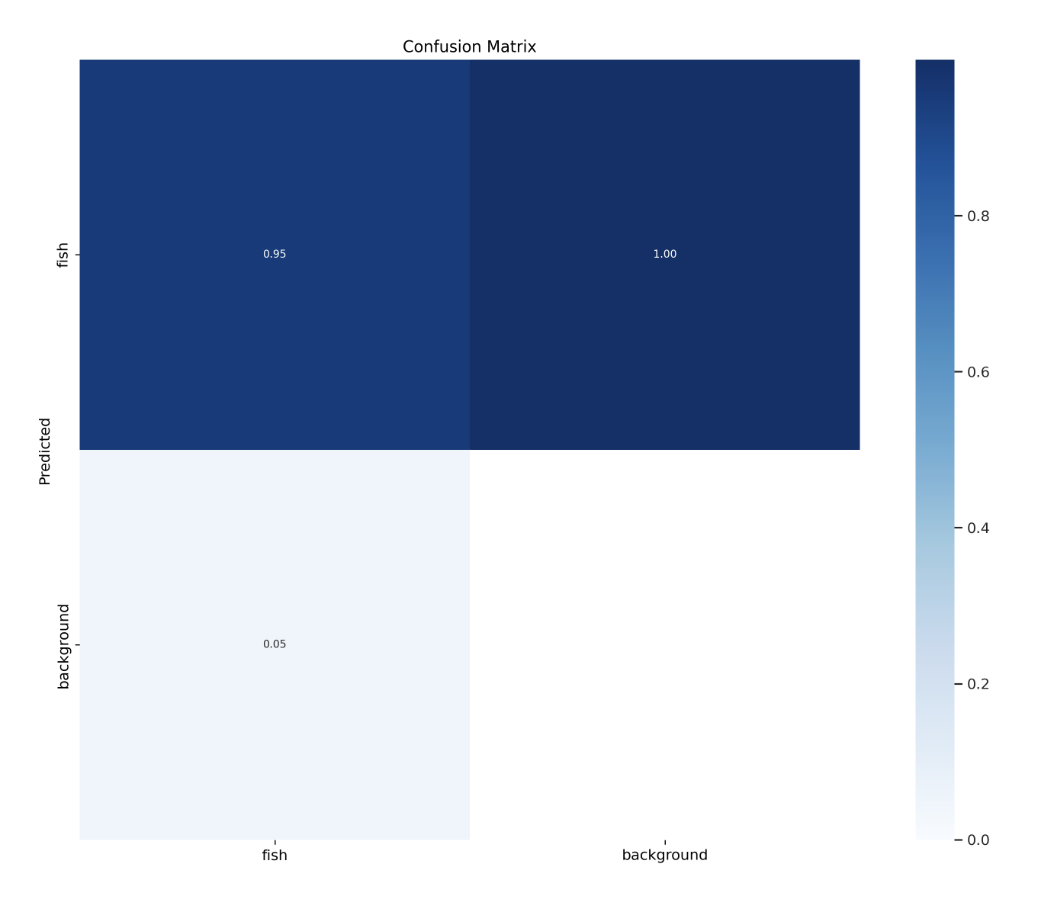
\includegraphics[height=0.9\textheight,width=0.9\textwidth,keepaspectratio]{images/1.png}
    

 \end{frame}

 \begin{frame}{Results}
    \centering
        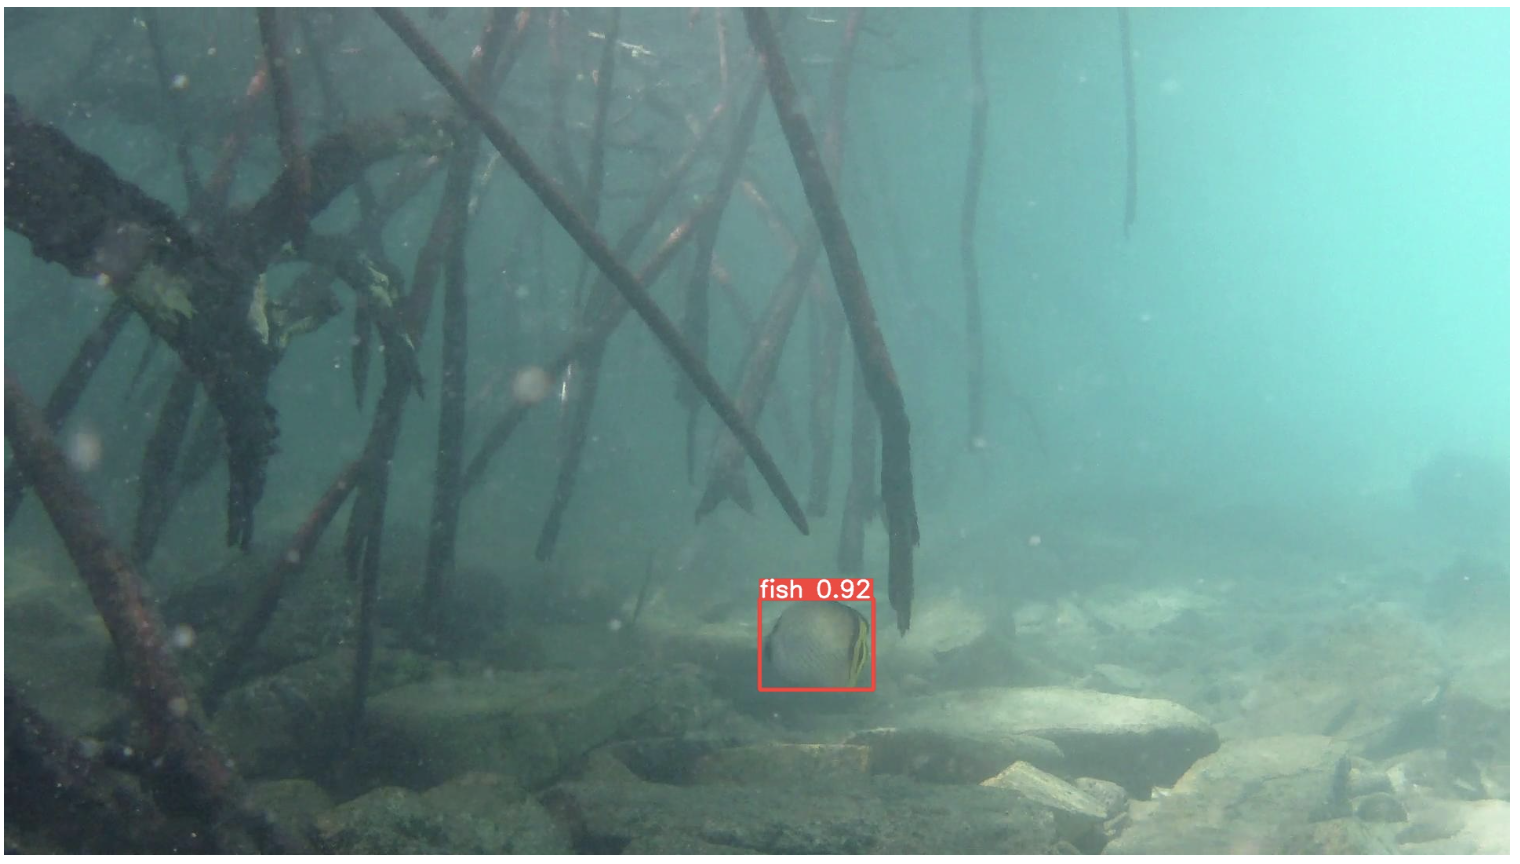
\includegraphics[height=0.7\textheight,width=0.7\textwidth,keepaspectratio]{images/2.png}
    

 \end{frame}

 \begin{frame}{Results}
    \centering
        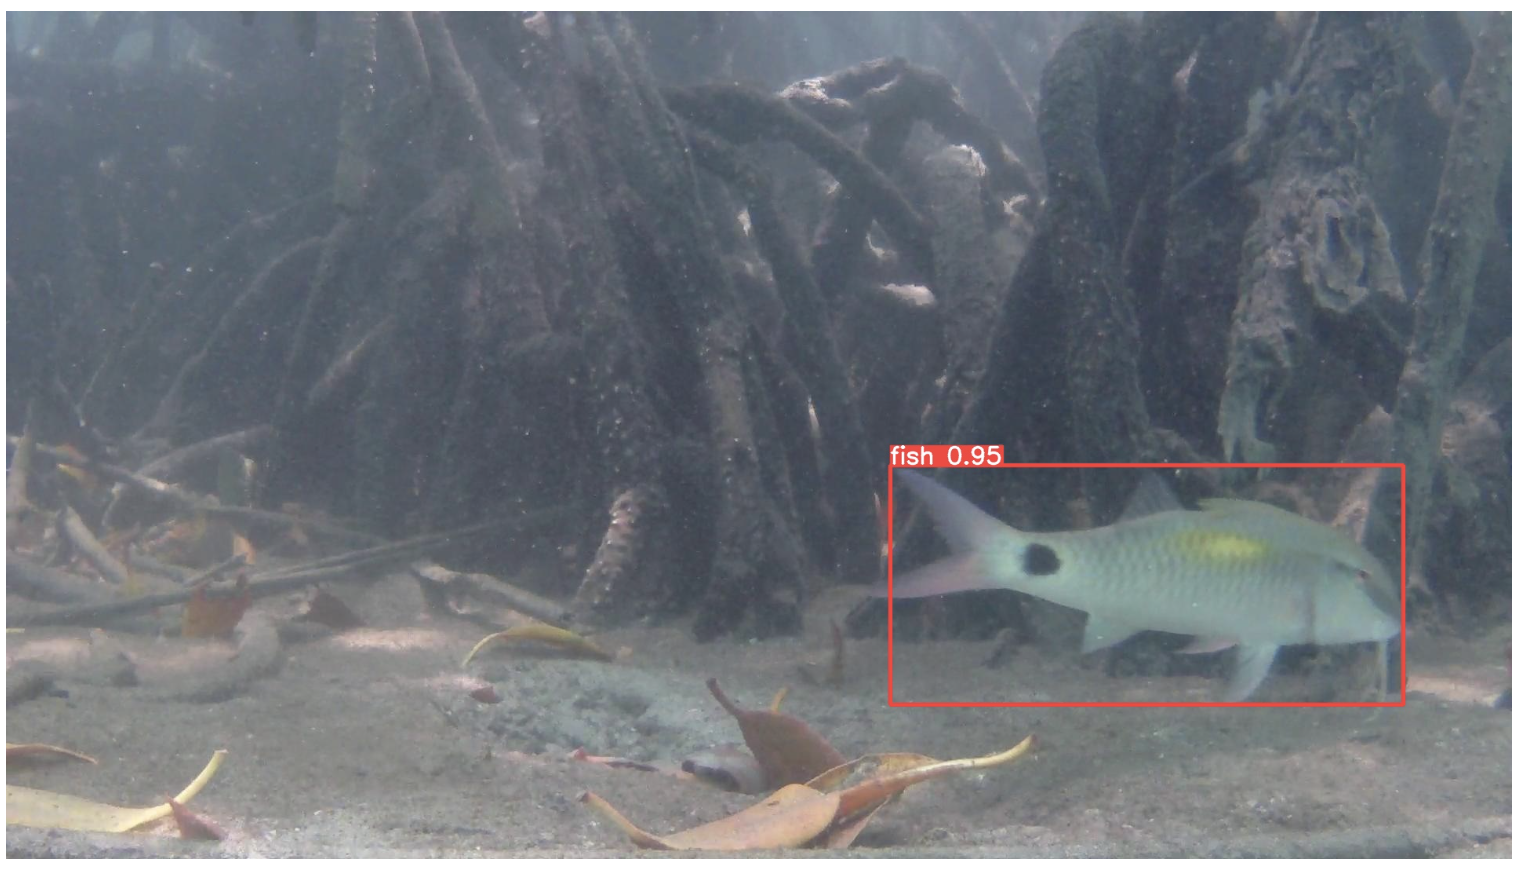
\includegraphics[height=0.7\textheight,width=0.7\textwidth,keepaspectratio]{images/3.png}
    

 \end{frame}

 \begin{frame}{Results}
    \centering
        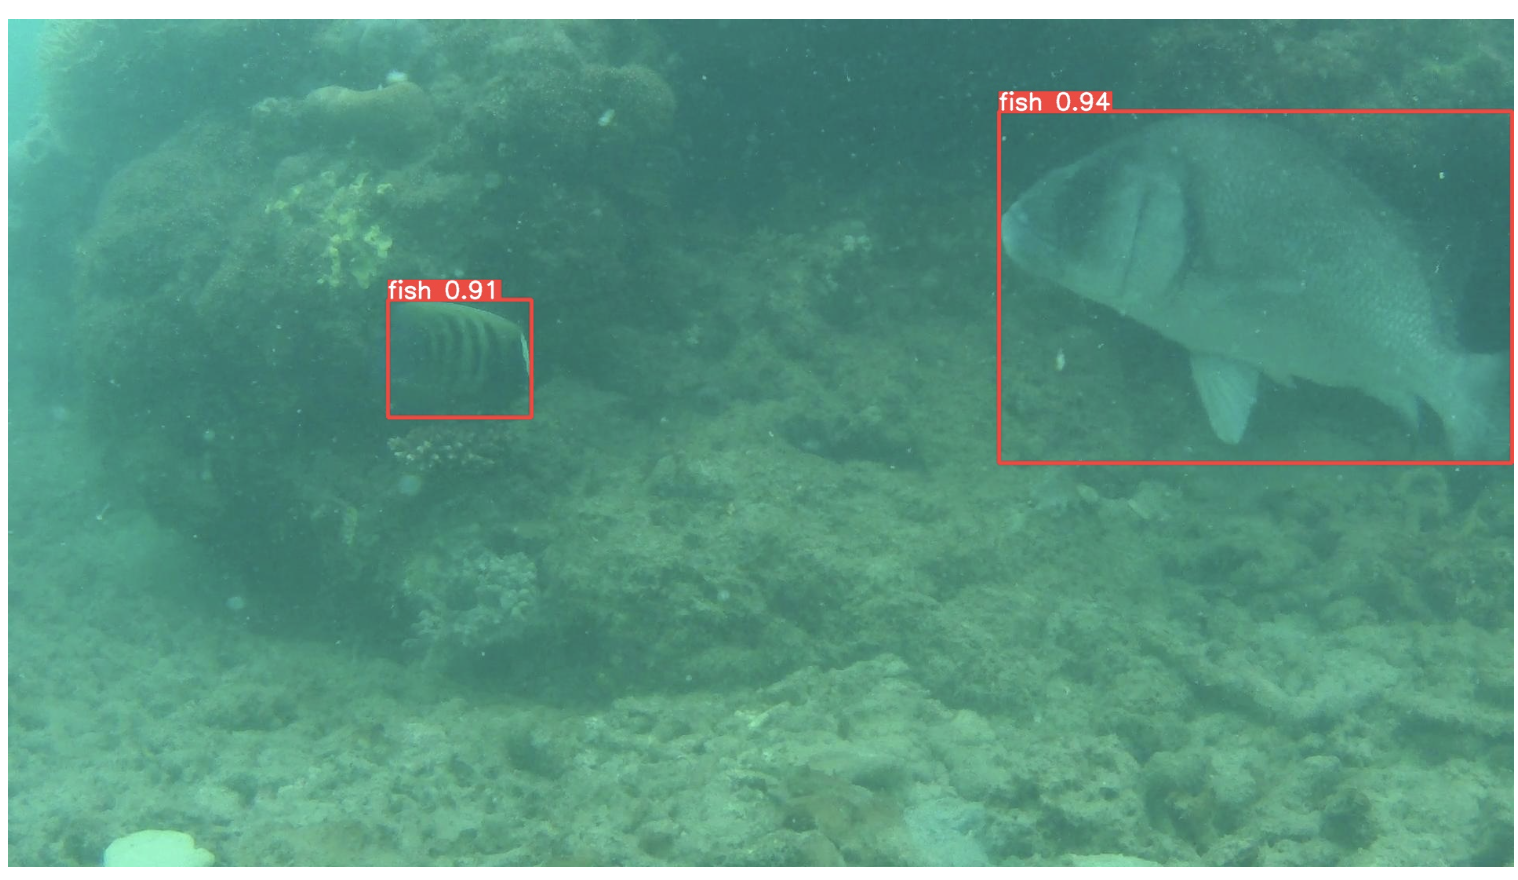
\includegraphics[height=0.7\textheight,width=0.7\textwidth,keepaspectratio]{images/4.png}
    

 \end{frame}

 \begin{frame}{Results}
    \centering
        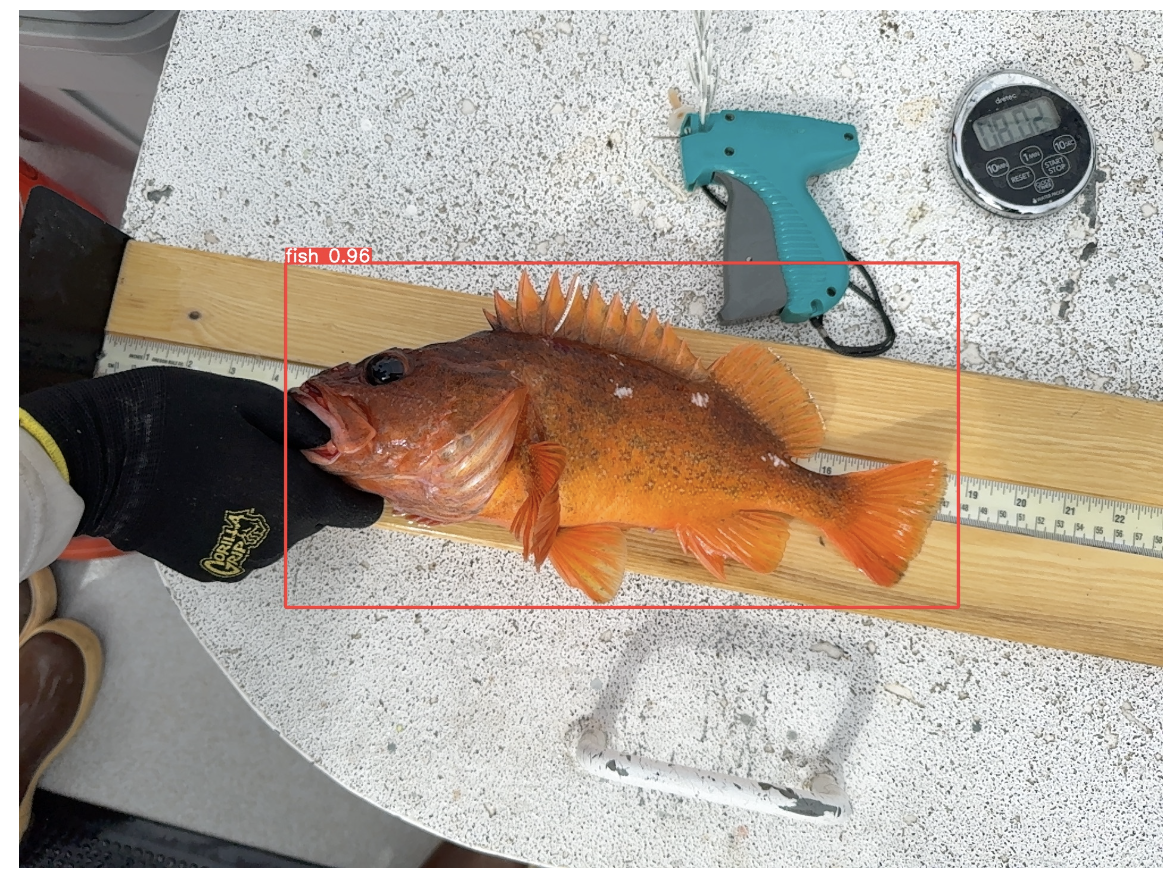
\includegraphics[height=0.7\textheight,width=0.7\textwidth,keepaspectratio]{images/5.png}
    

 \end{frame}

 \begin{frame}{Results}
    \centering
        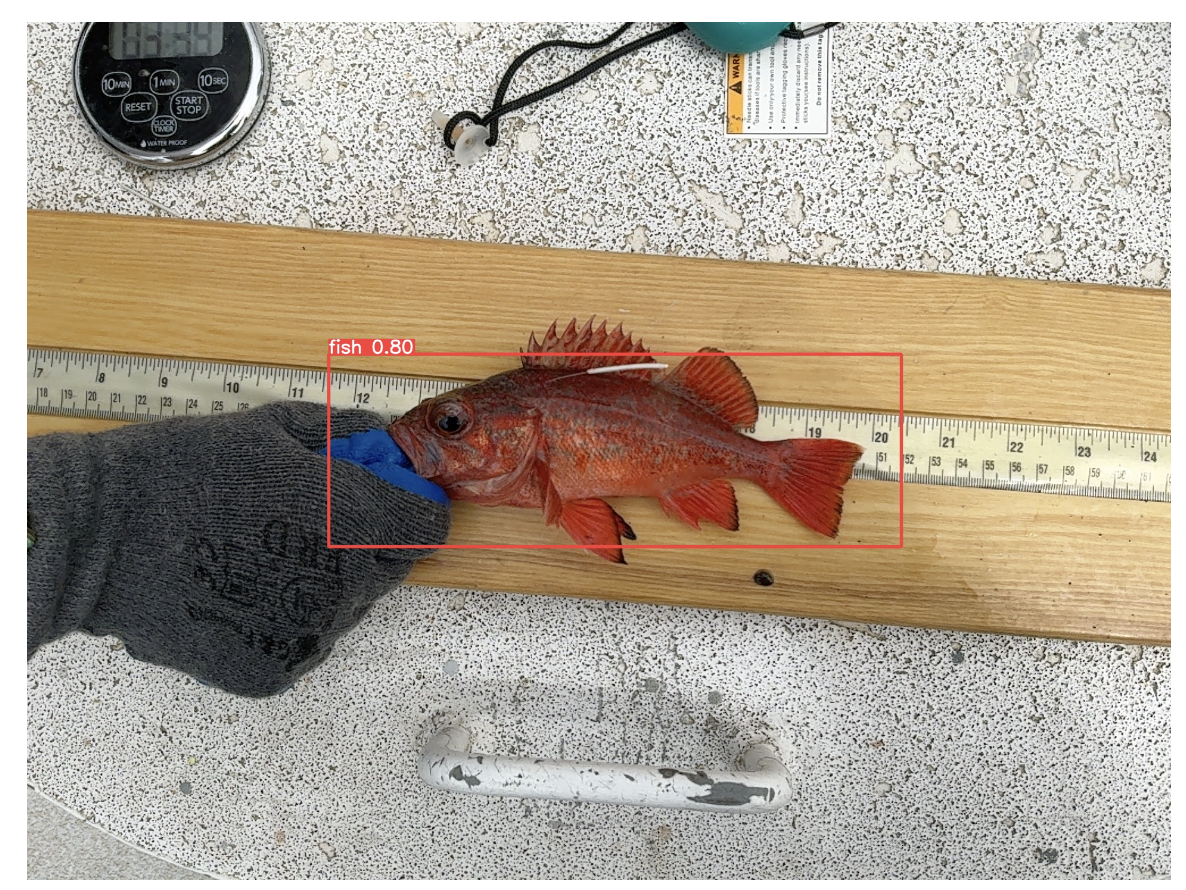
\includegraphics[height=0.7\textheight,width=0.7\textwidth,keepaspectratio]{images/6.png}
    

 \end{frame}
 \begin{frame}{Results}
    \centering
        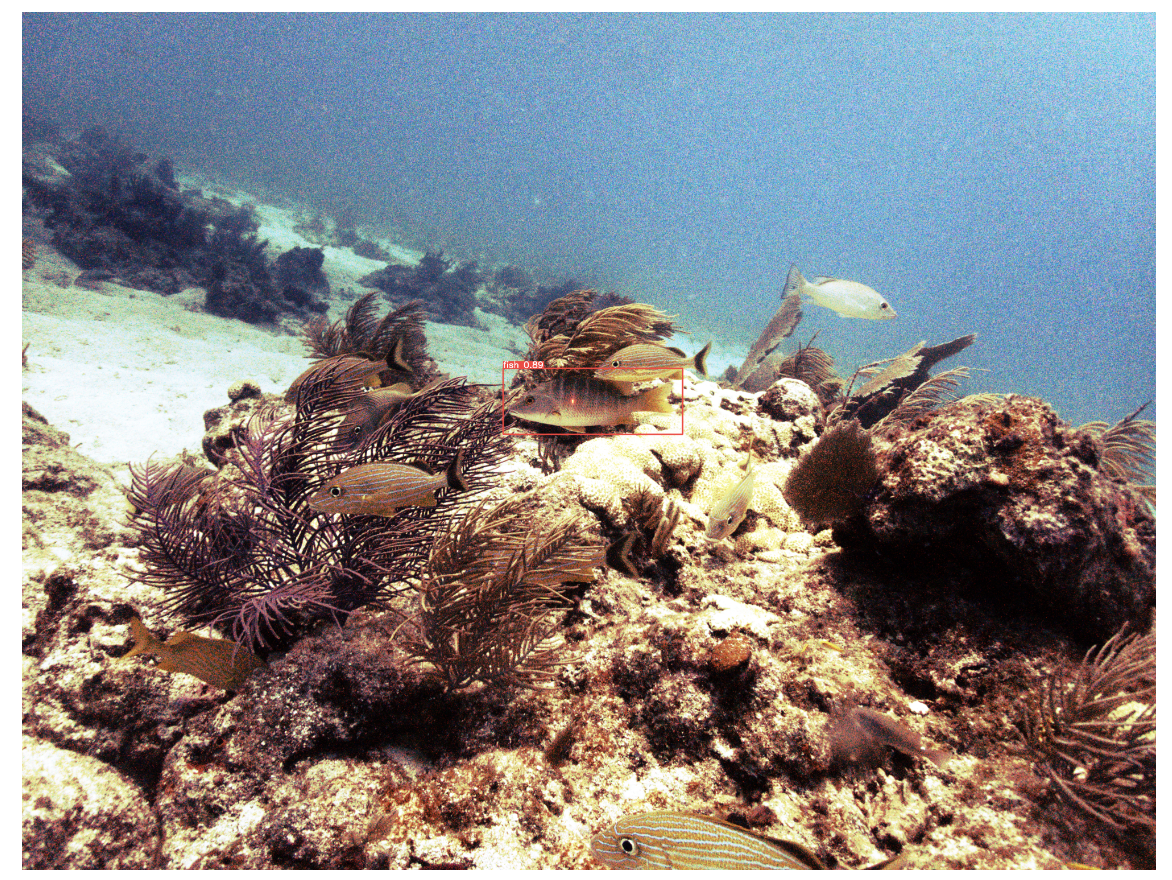
\includegraphics[height=0.7\textheight,width=0.7\textwidth,keepaspectratio]{images/7.png}
    

 \end{frame}

 \begin{frame}{Results}
   \begin{itemize}
      \item Some boxes failed to include the entire fish
      \item Poor performance on multi-instance images
   \end{itemize}
    



\end{frame}




\begin{frame}{Next Step}
   \begin{itemize}
      \item Fix problematic labels
      \item Integrate more training data 
   \end{itemize}
    

 \end{frame}
% To create a slide with a bullet list, use the following:
% \begin{frame}{TITLE}
%     \begin{itemize}
%         \item ITEM 1
%         \item ITEM 2
%     \end{itemize}    
% \end{frame}

% To create a slide with numbered list, use the following:
% \begin{frame}{TITLE}
%     \begin{enumerate}
%         \item ITEM 1
%         \item ITEM 2
%     \end{enumerate}
% \end{frame}

% To create a slide with a graphic:
% 1. Add the graphic to this folder (named picture.png)
% 2. Use the following:
% \begin{frame}{TITLE}
%     \centering
%     \includegraphics[height=0.7\textheight,width=0.7\textwidth,keepaspectratio]{picture.png}
% \end{frame}

% To create a slide with two columns, use the following:
% \begin{frame}{TITLE}
%     \begin{columns}
%         \begin{column}{0.5\textwidth}
%             COLUMN 1 BODY
%         \end{column}
%         \begin{column}{0.5\textwidth}
%             COLUMN 2 BODY
%         \end{column}
%     \end{columns}
% \end{frame}
